\documentclass{beamer}
\usepackage[utf8]{inputenc}
\usepackage{graphicx} % picturing
\usepackage{cite}
\usepackage{caption}
\usepackage{fancybox}
\usepackage{natbib}
\usepackage{cite}
\usepackage{animate}
\usepackage[utf8]{inputenc}
\usepackage[ngerman]{babel}
\usepackage{graphicx}
\usepackage{color}


%quotatation with source
\def\signed #1{{\leavevmode\unskip\nobreak\hfil\penalty50\hskip2em
  \hbox{}\nobreak\hfil(#1)%
  \parfillskip=0pt \finalhyphendemerits=0 \endgraf}}
\newsavebox\mybox
\newenvironment{aquote}[1]
  {\savebox\mybox{#1}\begin{quote}}
  {\signed{\usebox\mybox}\end{quote}}

\setbeamercovered{transparent}

%\usetheme{Pittsburgh}
\usetheme{AnnArbor}
%\usecolortheme{crane}
\usecolortheme{beaver}
\beamertemplatenavigationsymbolsempty
\setbeamertemplate{itemize items}[default]
\setbeamertemplate{enumerate items}[default]
\setbeamertemplate{sections/subsections in toc}[circle]
\setbeamercolor{section number projected}{bg=darkred,fg=white}
\setbeamercolor{enumerate item}{fg=darkred}
\setbeamercolor{enumerate subitem}{fg=darkred}
\setbeamercolor{enumerate subsubitem}{fg=darkred}
\setbeamercolor{itemize item}{fg=darkred}
\setbeamercolor{itemize subitem}{fg=darkred}
\setbeamercolor{itemize subsubitem}{fg=darkred}
\setbeamercolor{caption name}{fg=darkred}


\captionsetup[figure]{font=scriptsize}

\setbeamertemplate{footline}
  {%
    \begin{beamercolorbox}[ht=2.5ex,dp=1.125ex,%
      leftskip=.3cm,rightskip=.3cm plus1fil]{author in head/foot}%
      \leavevmode{\usebeamerfont{author in head/foot}\insertshortauthor}%
      \hfill%
      {\usebeamerfont{institute in head/foot}\usebeamercolor[fg]{institute in head/foot}\insertshortinstitute}%
    \end{beamercolorbox}%
    \begin{beamercolorbox}[ht=2.5ex,dp=1.125ex,%
      leftskip=.3cm,rightskip=.3cm plus1fil]{title in head/foot}%
      \leavevmode{\usebeamerfont{title in head/foot}\insertshorttitle}%
      \hfill%
      %{\usebeamerfont{pagecounter in head/foot}\usebeamercolor[fg]{pagecounter in head/foot}\[~\thepage\]}%
      {\usebeamerfont{pagecounter in head/foot}\usebeamercolor[fg]{pagecounter in head/foot}\lbrack~\insertframenumber~\rbrack}%
    \end{beamercolorbox}%
    \begin{beamercolorbox}[colsep=1.5pt]{lower separation line foot}	
    \end{beamercolorbox}
  }


\title[BacArena]{\texttt{BacArena}: Simulation of Interactions in Microbial Communities using Genome-wide Metabolic Reconstructions}
  \author[Eugen Bauer, Johannes Zimmermann]{Eugen Bauer, Johannes Zimmermann\\ \small{\{eugen.bauer, zimmermann.johannes\}@uni-jena.de}}
\institute{Universit\"at Jena}
\date{23.10.2013}
\begin{document}


\frame{
\titlepage
}

\frame{
  \title{Agent based modeling}
}

\frame{
  \title{Constrained based modeling}
}

\frame{
  \title{Reproducible Simulations}
}

\frame{
  \title{Modularity}
}


\frame{
\begin{figure}[h!]
  \centering
    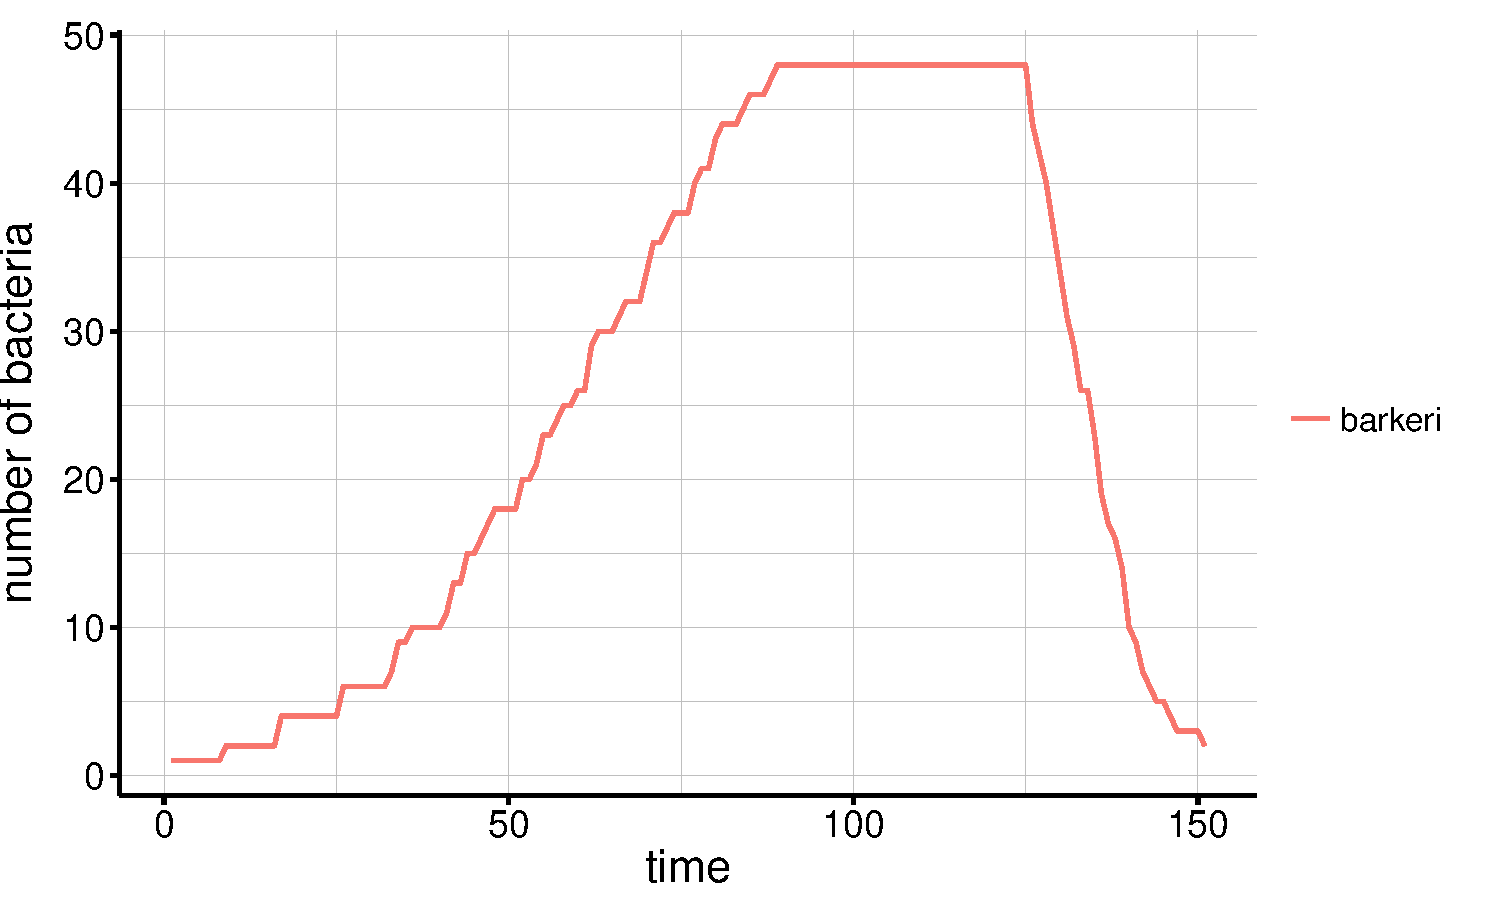
\includegraphics[scale=0.4]{../results/img/barkeri_20x20_seed9659_growth.pdf}
    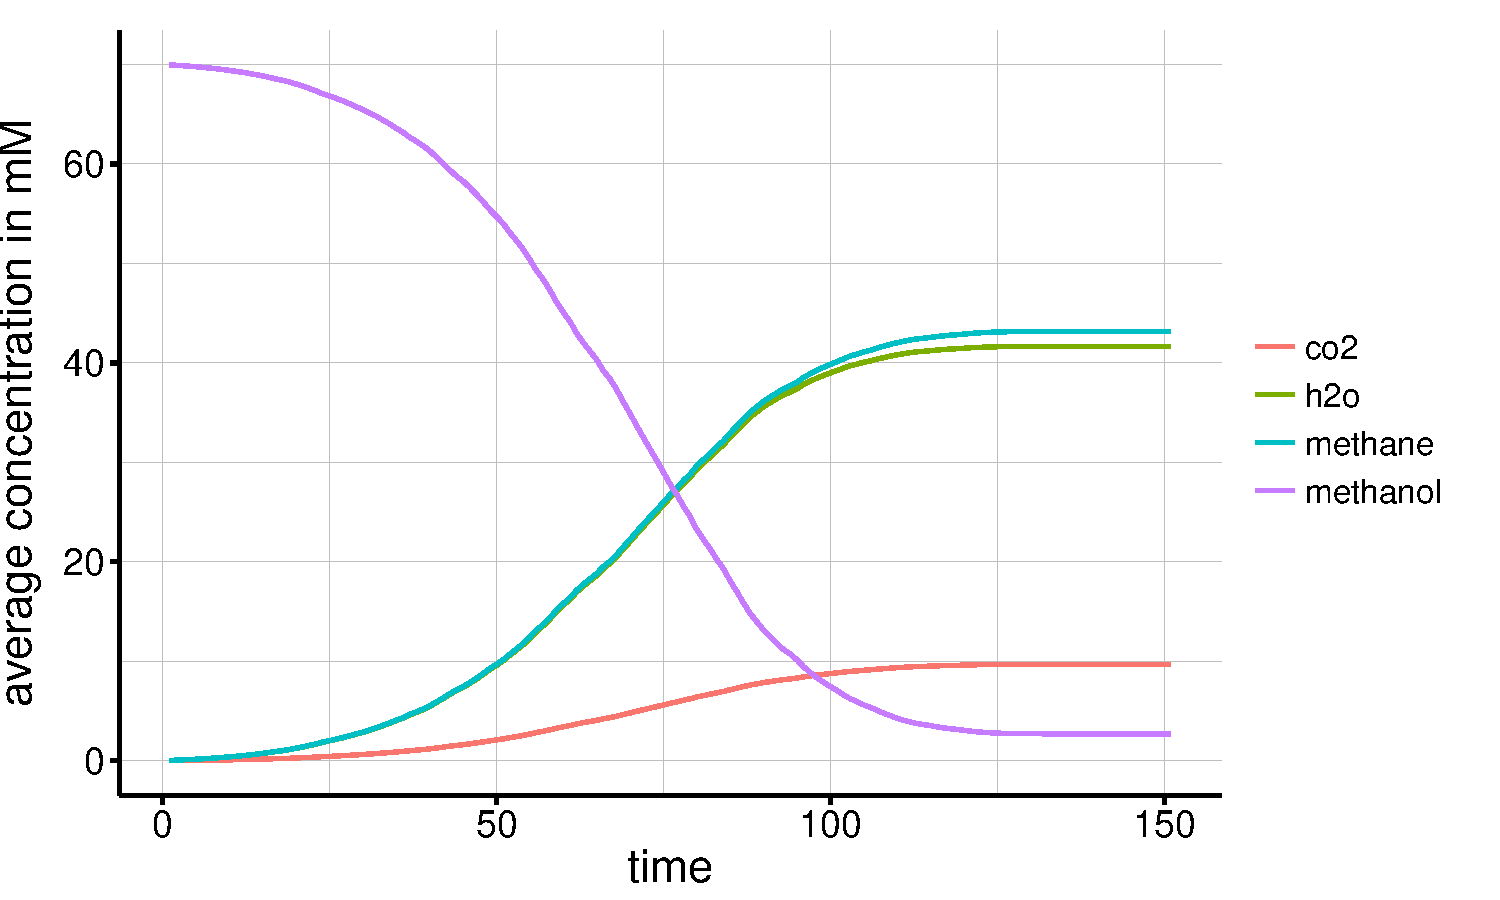
\includegraphics[scale=0.4]{../results/img/barkeri_20x20_seed9659_subs.pdf}
  \caption{Population dynamics of the \emph{M. barkeri} model on a $20\times20$ grid, with bacterial growth (A) and consumption/production of various metabolites (B). An initial concentration of 70\;mmol per grid cell of methanol was added to the environment. The seed of the random number generator was set to 9659.}
  \label{fig:barkerisg}
\end{figure}
\begin{figure}[h!]

  \centering
  \subfigure[]{
    \begin{minipage}[t]{0.3\textwidth}
    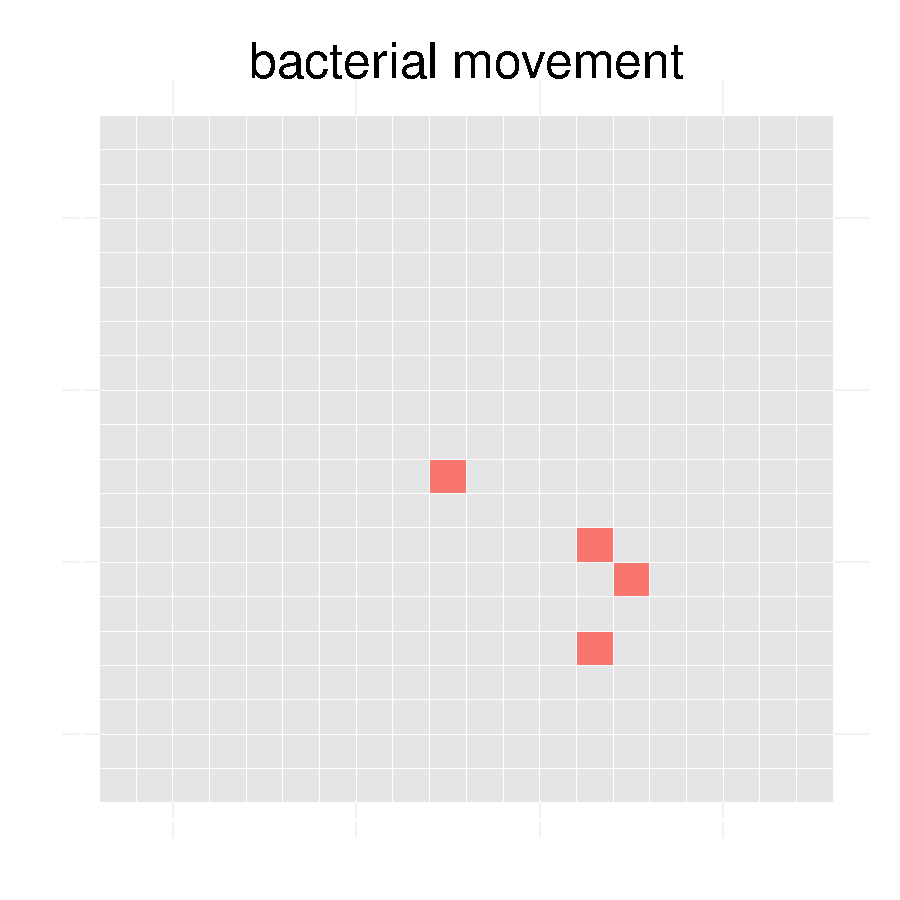
\includegraphics[width=\textwidth]{../results/img/barkeri_20x20_seed9659_bac25.pdf}
  \end{minipage}
  \begin{minipage}[t]{0.3\textwidth}
    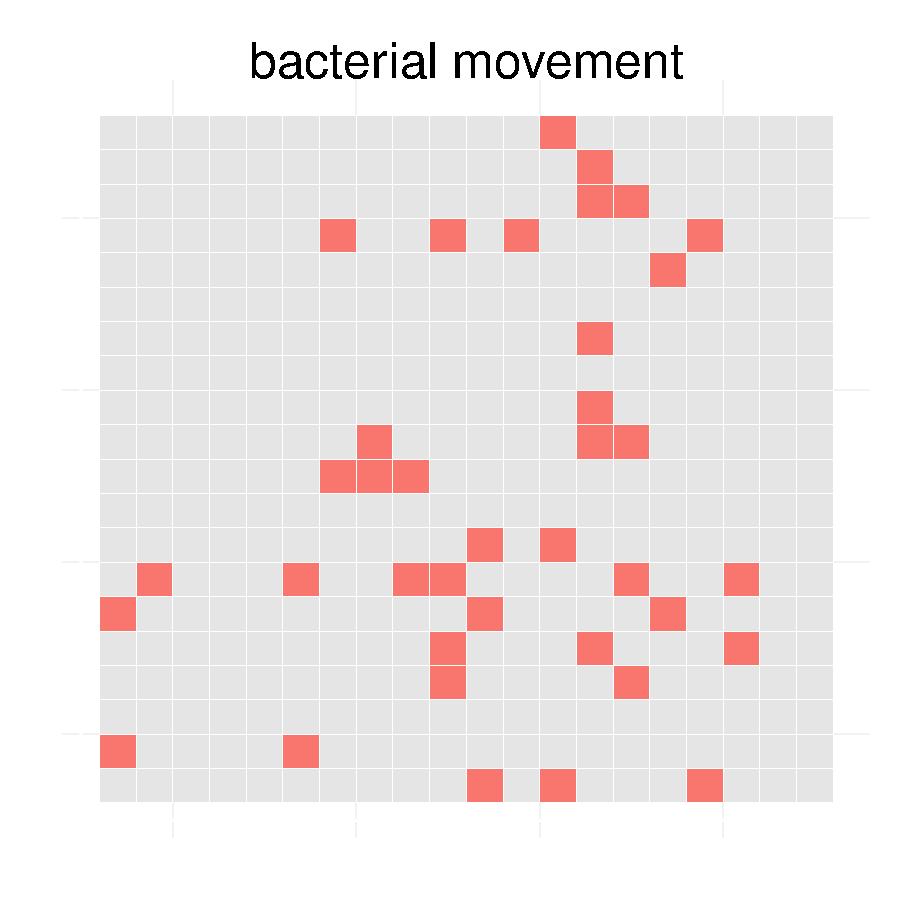
\includegraphics[width=\textwidth]{../results/img/barkeri_20x20_seed9659_bac75.pdf}
  \end{minipage}
  \begin{minipage}[t]{0.3\textwidth}
      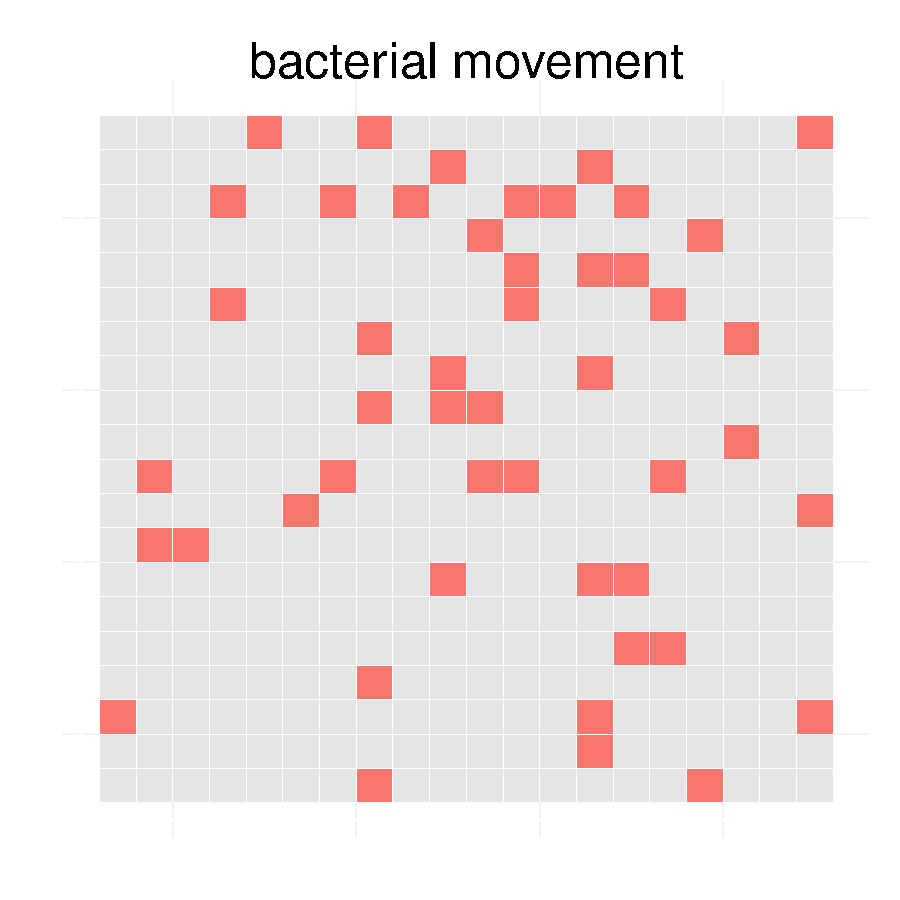
\includegraphics[width=\textwidth]{../results/img/barkeri_20x20_seed9659_bac100.pdf}
  \end{minipage}
  }
  \subfigure[]{
  \begin{minipage}[t]{0.3\textwidth}
    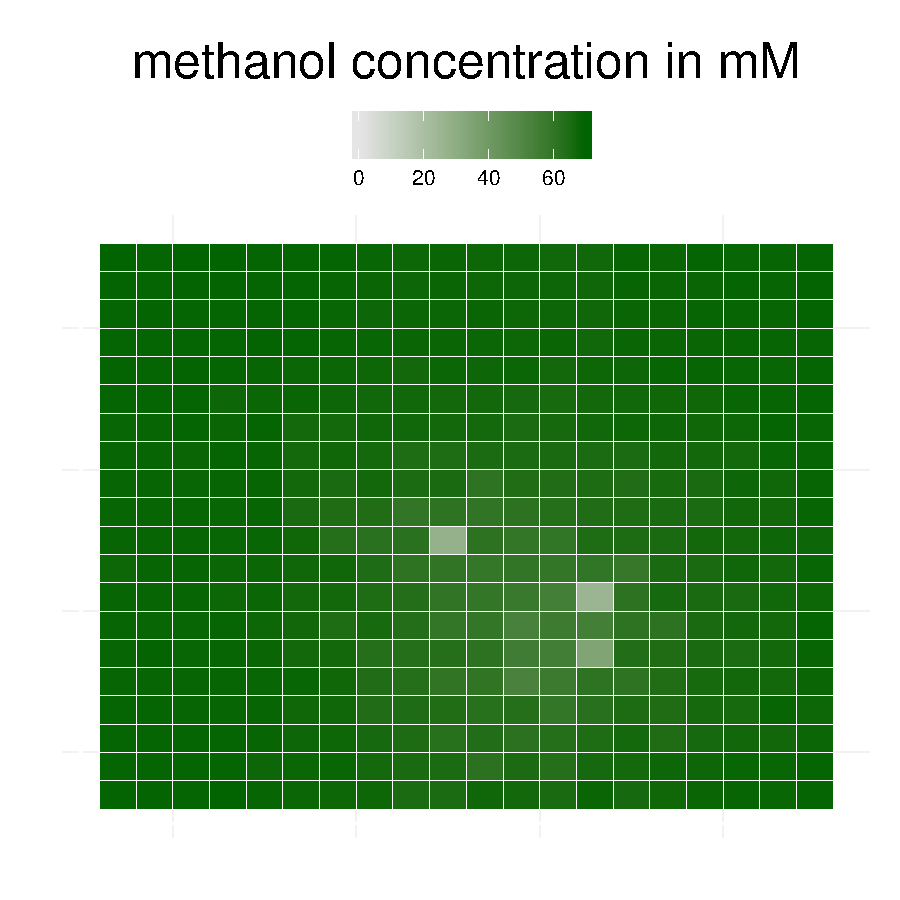
\includegraphics[width=\textwidth]{../results/img/barkeri_20x20_seed9659_meth25.pdf}
  \end{minipage}
  \begin{minipage}[t]{0.3\textwidth}
    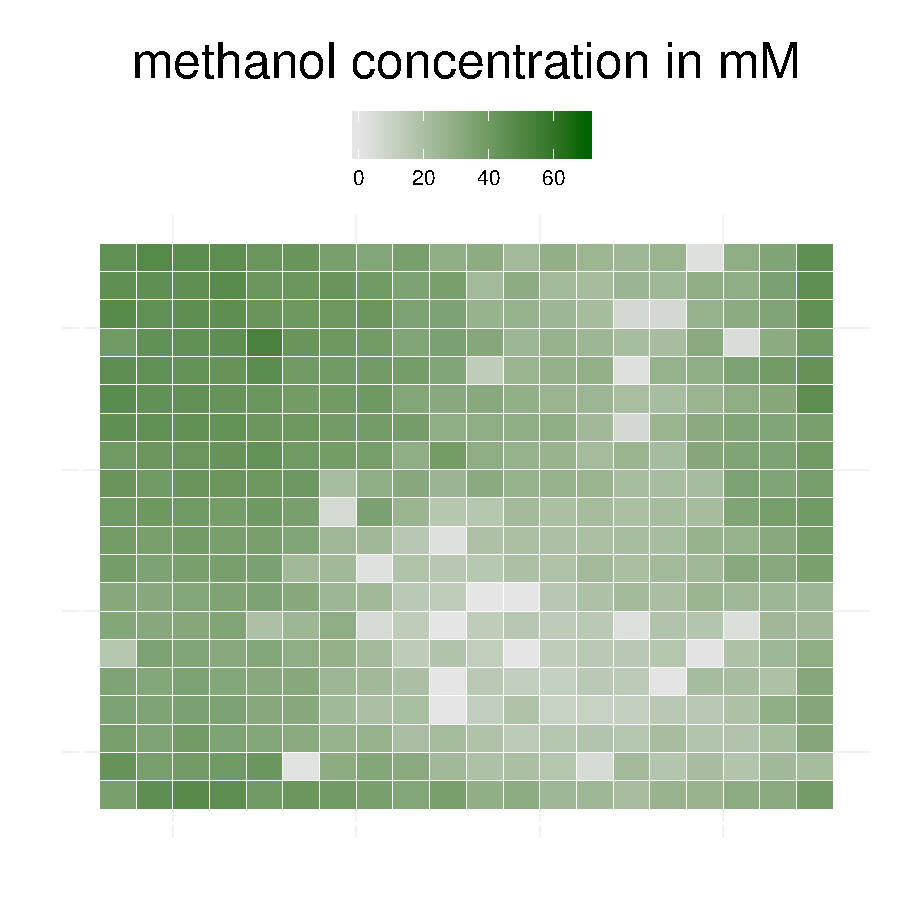
\includegraphics[width=\textwidth]{../results/img/barkeri_20x20_seed9659_meth75.pdf}
  \end{minipage}
  \begin{minipage}[t]{0.3\textwidth}
    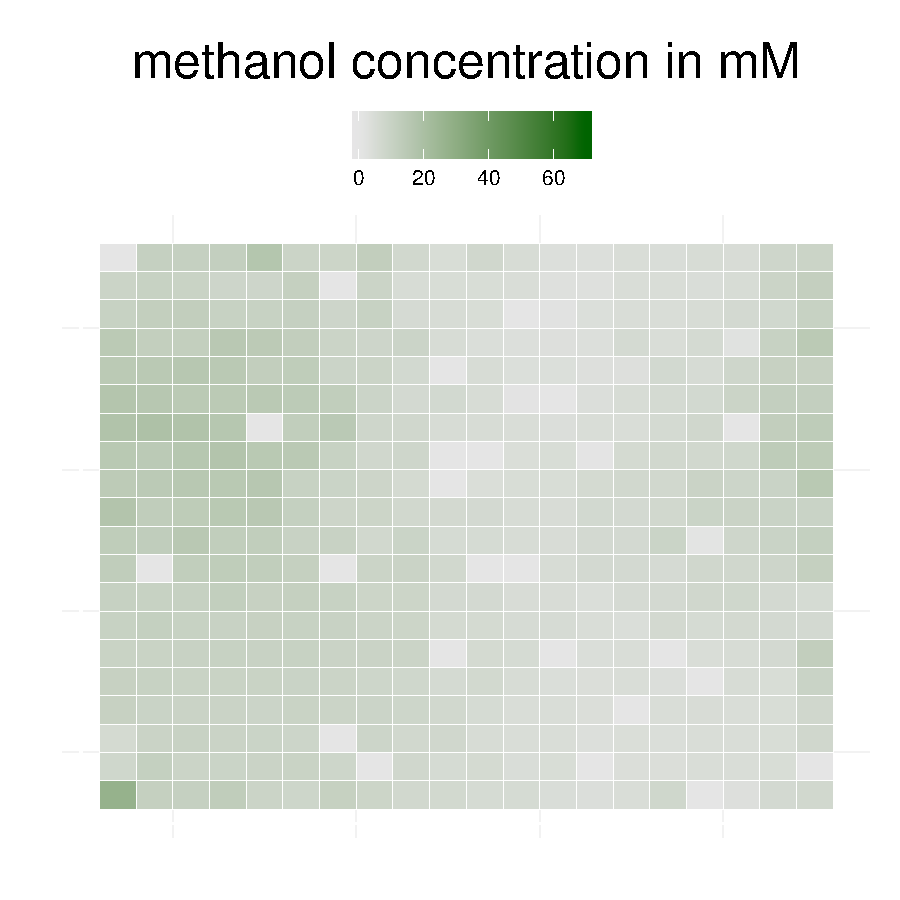
\includegraphics[width=\textwidth]{../results/img/barkeri_20x20_seed9659_meth100.pdf}
  \end{minipage}
  }
  \subfigure[]{
  \begin{minipage}[t]{0.3\textwidth}
    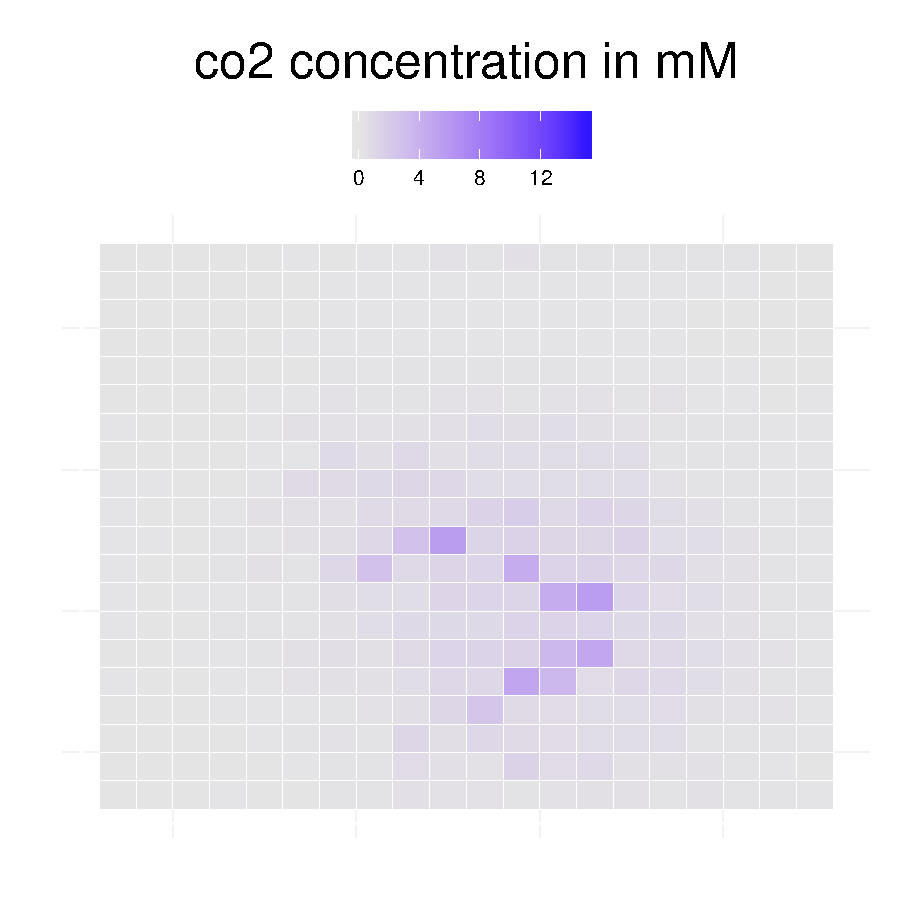
\includegraphics[width=\textwidth]{../results/img/barkeri_20x20_seed9659_co225.pdf}
  \end{minipage}
  \begin{minipage}[t]{0.3\textwidth}
    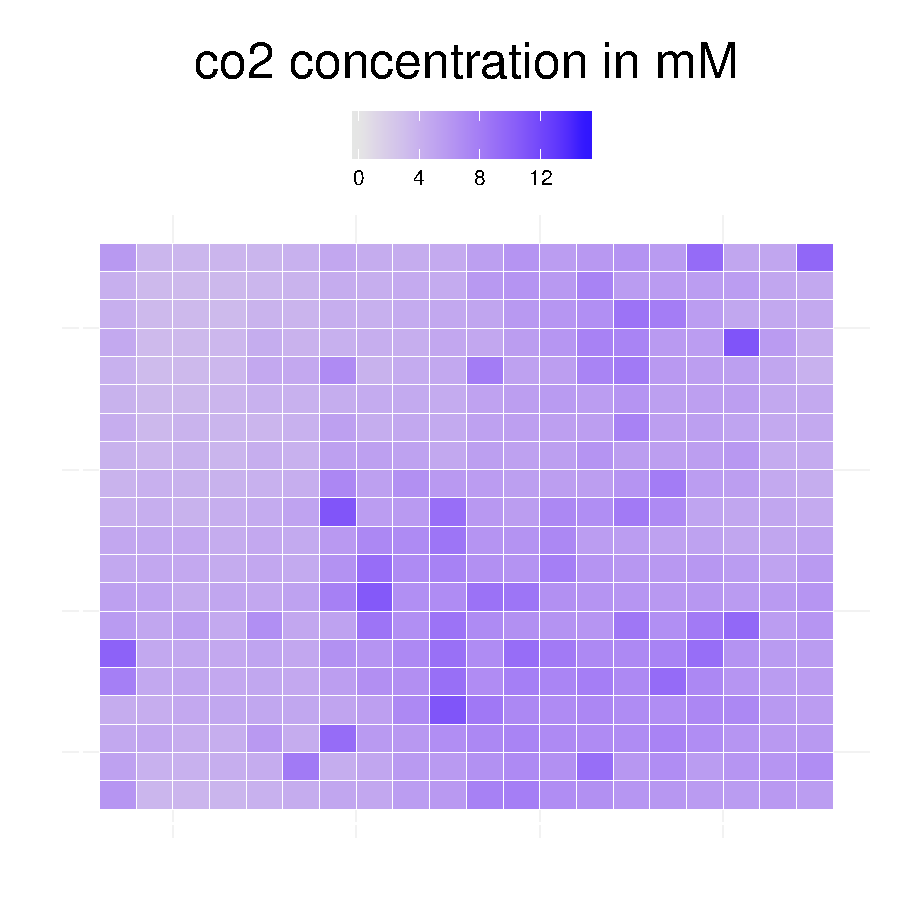
\includegraphics[width=\textwidth]{../results/img/barkeri_20x20_seed9659_co275.pdf}
  \end{minipage}
  \begin{minipage}[t]{0.3\textwidth}
    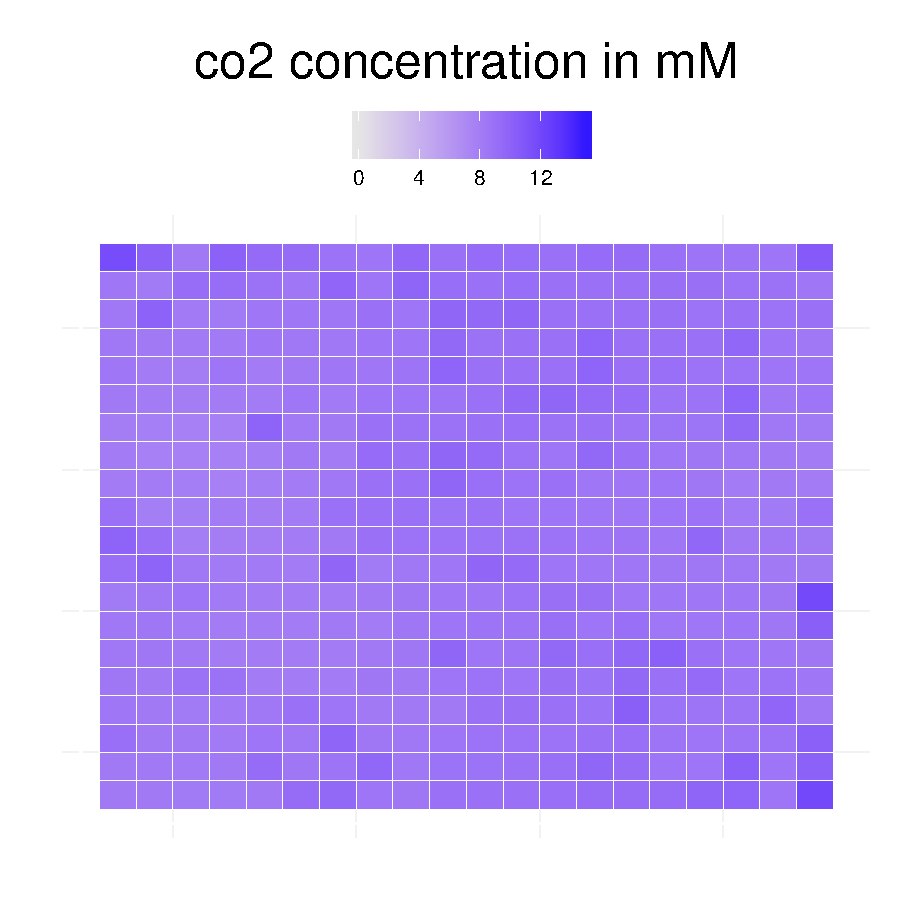
\includegraphics[width=\textwidth]{../results/img/barkeri_20x20_seed9659_co2100.pdf}
  \end{minipage}
  }
  \subfigure[]{
  \begin{minipage}[t]{0.3\textwidth}
    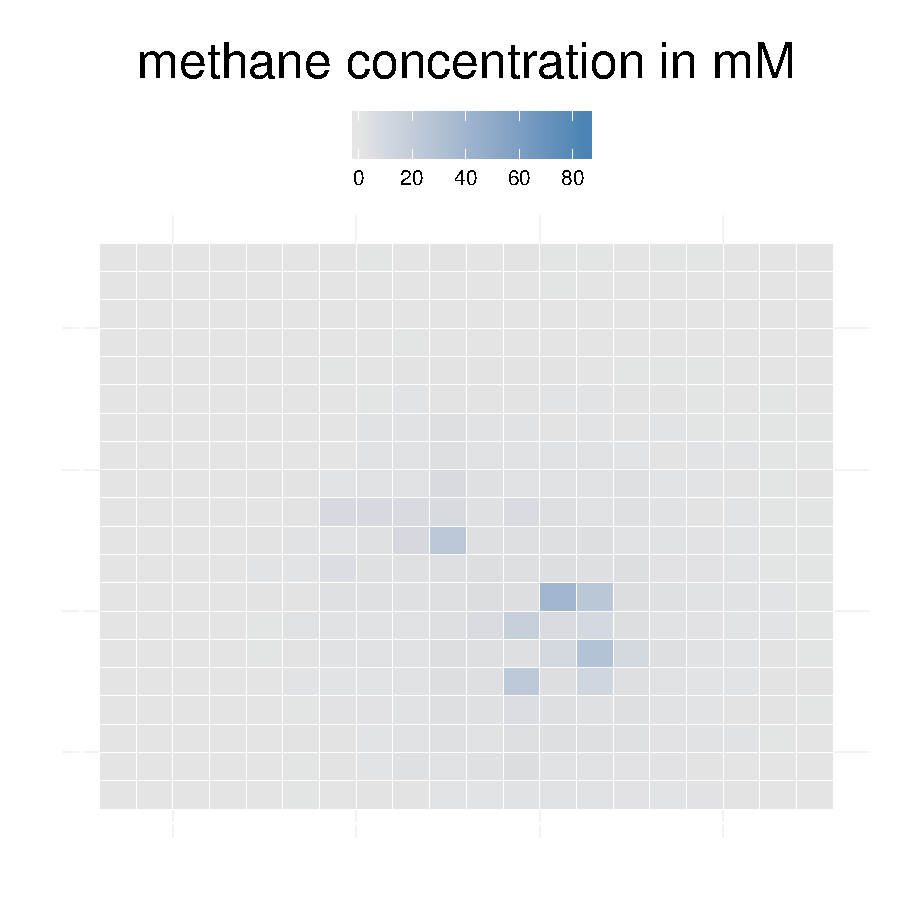
\includegraphics[width=\textwidth]{../results/img/barkeri_20x20_seed9659_methane25.pdf}
  \end{minipage}
  \begin{minipage}[t]{0.3\textwidth}
    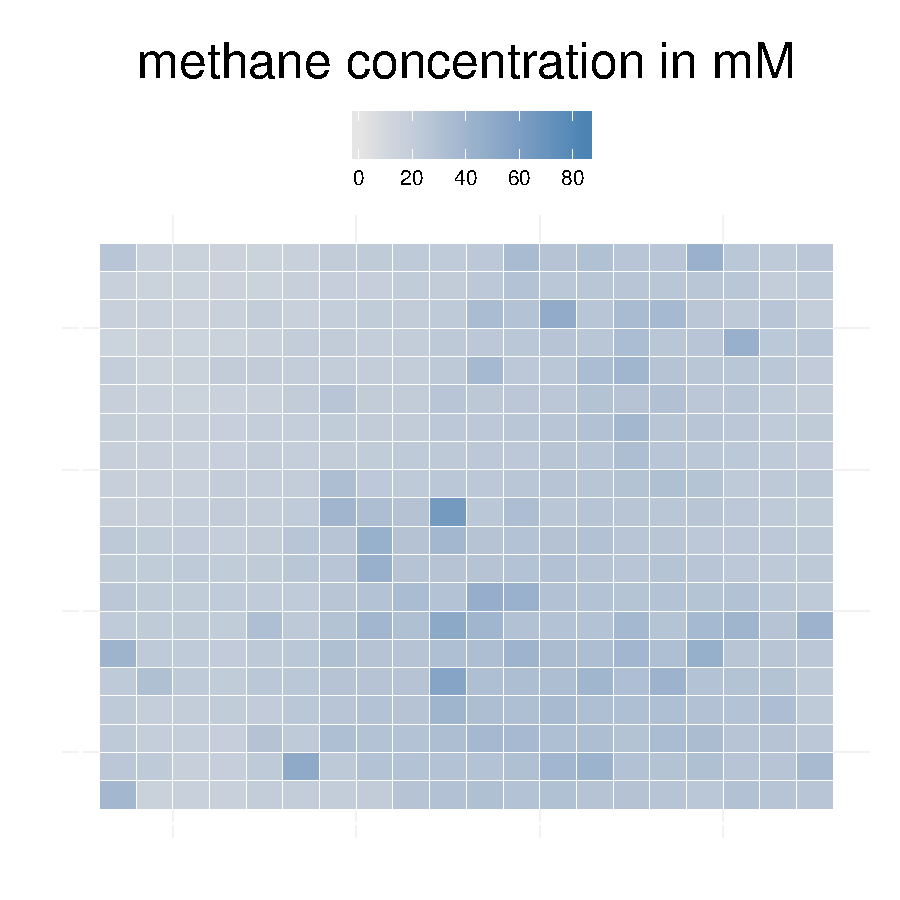
\includegraphics[width=\textwidth]{../results/img/barkeri_20x20_seed9659_methane75.pdf}
  \end{minipage}
  \begin{minipage}[t]{0.3\textwidth}
    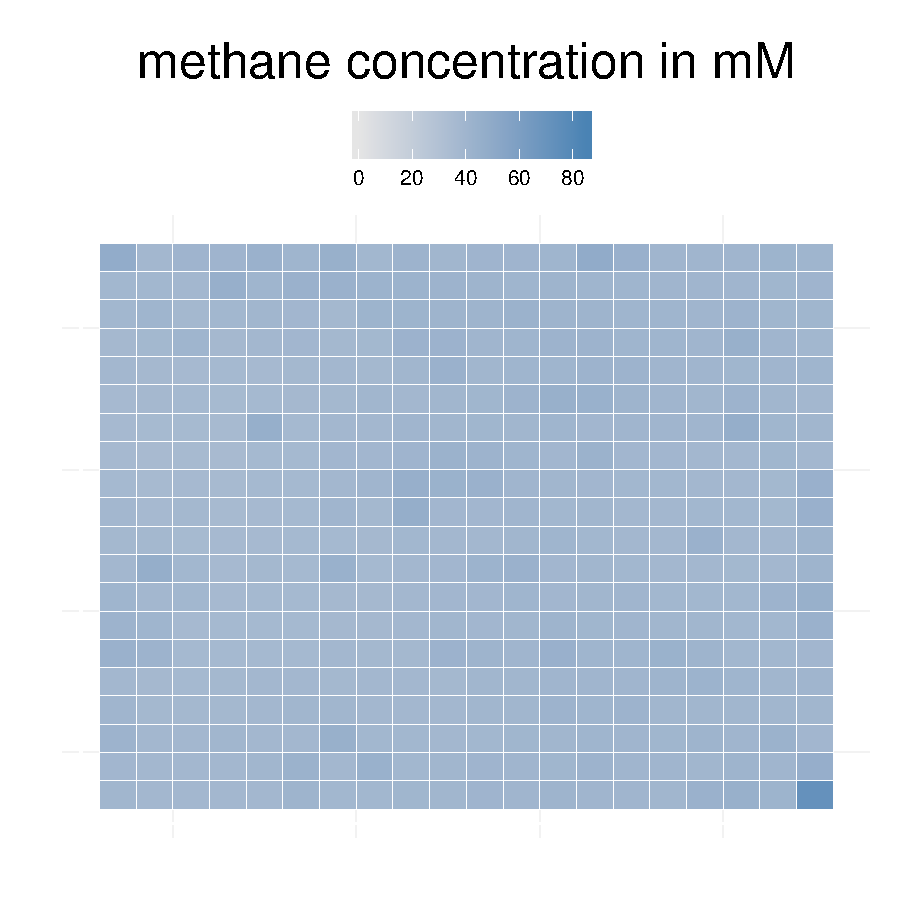
\includegraphics[width=\textwidth]{../results/img/barkeri_20x20_seed9659_methane100.pdf}
  \end{minipage}
  }
  \caption{Population dynamics of the \emph{M. barkeri} model on a $20\times20$ grid, with bacterial movement (A) and concentrations of methanol (B), CO$_2$ (C) and methane (D) (of time step 25, 75 and 100). The seed of the random number generator was set to 9659.}
  \label{fig:barkerigrids}
\end{figure}
}

\end{document}
\frame{
  \frametitle{}
}
  \begin{figure}
    \centering
    \includegraphics[height=0.85\textheight]{./bacarena1.pdf}
  \end{figure}
}
\frame{
  \frametitle{BacArena: Methanosarcina barkeri}
  \begin{figure}
    \centering
    \includegraphics[height=0.85\textheight]{./bacarena2.pdf}
  \end{figure}
